\chapter{Marco Teórico}\label{mt}
\section{Estado del Arte}
    \par Para el desarrollo de este trabajo se hizo una investigación sobre los sistemas que solucionan problemas similares y a que objetivos responden. Al mismo tiempo como abordar el hecho de que el usuario es parte fundamental del flujo del sistema tanto en su funcionamiento como imponiendo restricciones dinámicas sobre el mismo, las que responderían a preferencias o valores de cada usuario\footnote{Esto se extrae del trabajo con alumnos, ver \ref{sec:focus}}. Por este motivo los temas abordados e investigados a continuación son \textit{\acrfull{UCD}}, \textit{human in the loop}, \textit{information systems} y \textit{chatbots}.
    
    \subsection{Requisitos diseño centrado en el usuario}
    \par Este es un sistema que indudablemente se basa en el usuario y sus preferencias, es por esta razón que para que el desarrollo sea exitoso no basta con que se desarrolle de la manera correcta y asumiendo buenas prácticas, sino que debe hacerse en torno al usuario y rescatando no solo su input \cite{Karat1997}, sino sus objetivos y valores. Dentro de las maneras de enfocar un desarrollo centrado en el usuario encontramos 3 alternativas la especialista, generalista y mixto \cite{Fox2008}.
    \par La manera especialista hace referencia a que hay 3 actores encargados del proceso, los usuarios, los encargados de \acrshort{UCD} y el resto del equipo de desarrollo. Por otro lado, la generalista asume dos roles: el de usuario y el de desarrollador encargado de esta área.
    \par En esta línea de \textit{\acrlong{UCD}}, el diseño propiamente tal, se entiende como un proceso, en el que debe estar involucrado el usuario final, de forma constante.
    De modo que la personalización llega a ser \guillemotleft una pieza fundamental del diseño exitoso es aterrizar el desarrollo de \textit{features} y herramientas sobre el valor del usuario final\guillemotright \cite{Kramer2000}.
    \par De aquí se obtiene que el sistema debería ser personalizable, y rescatar lo que sea valorado por los usuarios. Dada la naturaleza del proyecto, se decide adoptar un enfoque generalista.
    
    \subsection{El usuario como input del sistema}
    \par Al ser un sistema que depende del usuario para determinar el curso de acción, el humano en este sistema no solo está en ciertos momentos críticos del flujo, sino que es el centro del flujo de información, modelos como este han sido validados con buenos resultados \cite{Smith2018} recientemente.
    \par Los sistemas de información asociados a chatbots, generalmente buscan la integración de información, este proceso es decir mostrarle al usuario una gran variedad de información de diferentes fuentes a través de una vista unificada viene asociado a varias dificultades técnicas y teóricas \cite{Li2017}.
    \par En este sentido, se propone que los sistemas de información que dependen de un humano son altamente complejos, porque los humanos, en este caso usuarios no solo son observadores, sino que tienen la capacidad de incidir en el ambiente no solo reaccionar al ambiente \cite{McBride2021}, sería iluso desarrollar un sistema para las personas sin considerar los objetivos de ellas de forma explícita en el diseño del sistema.
    \par Estos descubrimientos e investigaciones ponen varias restricciones en cuanto al desarrollo de un sistema que depende los usuarios para funcionar y que al mismo tiempo está centrado en el usuario. Pero las podemos condensar en al menos 2: El diseño del sistema debe considerar de forma explícita los objetivos del usuario en cada interacción y debe integrar la información.

    \subsection{Otras aplicaciones de los chatbots en el ámbito académico}
    \par Los chatbots se utilizan desde hace varios años para variados y diversos fines, en múltiples áreas. En particular ahora los abordaremos desde la esfera académica, centrándonos específicamente en instituciones de educación superior.
    En estas se utilizan principalmente como un medio de apoyo al proceso de aprendizaje, como soporte para procesos universitarios, como ayuda para la gestión académica y cómo un sistema de consulta que responde a dudas de diversos entes de estas instituciones.
    \par Como apoyo al proceso de aprendizaje los chatbots se han usado tanto dentro como fuera de la sala de clases.
    \par En la \textit{University of Salerno}, se creó un sistema para responder de manera efectiva las preguntas de los estudiantes, el contexto de \textit{e-learning}. A grandes rasgos es un sistema que usa procesamiento de lenguaje natural como técnicas de ontología, para ligar las preguntas de los estudiantes al contenido disponible y de esta forma poder responder eso que los alumnos están buscando \cite{Clarizia2018}.
    \par El Dr. Sherif Abdelhamid del \textit{Virginia Polytechnic Institute and State University} también propuso un sistema de características similares \cite{Abdelhamid2020}, con las distinciones de que uso el sistema de reconocimiento de voz para traducir las dudas verbales de los estudiantes a texto y así procesarlas y que su objetivo estaba ligados a los elementos que acompañaban el estudio más que al aprendizaje académico en sí. Algunos ejemplos como cuál es la bibliografía pertinente al curso, que recursos tiene disponibles, que debería aprender, etc.
    \par En este aspecto, investigadores del \textit{Department of Mathematics and Computer Science, University of Kabianga, Kericho, Kenya} con miembros del \textit{Department of Curriculum Instruction Educational Media, School of Education, Moi University, Kenya} analizaron la respuesta de los mismos profesores a la introducción de estas herramientas en la rutina de enseñanza \cite{K2018}.
    
    \par Como soporte para procesos universitarios los chatbots se han usado para entregar el horario de clases o las clases siguientes así cómo ayudar a los alumnos a elegir ramos.
    
    \par Desarrolladores de la \textit{Bogdan Khmelnytsky Melitopol State Pedagogical University} en Ucrania, desarrollaron un servicio de 3 capas para poder implementar un servicio de ayuda al entregar el horario de clases a través de un chatbot, esto se hacía no solo con la finalidad de ayudar a alumnos que hayan olvidado o no un horario o su sala, sino también porque los horarios pueden sufrir cambios o modificaciones, además de que si bien hay alternativas simples como fotos estas se pierden en un gran volumen de elementos similares sin relación, lo que las hace difícil de volver a obtener, según la investigación \cite{Priadko2019}.
    
    \par En \textit{The Open University of Hong Kong Hong Kong} desarrolladores implementaron un sistema para facilitar a los alumnos la decisión sobre qué cursos tomar a través de un chatbot \cite{ChunHo2018}.
    
    \par En el área de los desarrollos de ayuda para la gestión académica, se encontraron desarrollos ligados a: Hacer disponibles servicios en horarios no hábiles, Mantener, monitorear y mostrar la información del alumno y Acercar la implementación de chatbots a usuarios de más alto nivel y con menos conocimiento técnico.
    
    \par Los trabajos de Vaishnavi Ajay Inamdar1 y Shivanand R.D en el \textit{BIET College} de la India, van enfocados en poder proveer servicios de gestión académica en cualquier momento, de este modo bajar la carga de los funcionarios y proveer de una \textit{\gls{effectiveGUI}} \cite{Journal2019}.
    
    \par Del \textit{Engineering Rajalakshmi Institute of Technology} una profesora y sus alumnos, desarrollaron un sistema para administrar la información escolar de los alumnos y está ligado la base de datos de administración. Este sistema tenía el foco en el personal administrativo de la institución y dependía de la información entregada por el alumno.
    
    \par Con el foco en los apoderados o tutores de un alumno, en la \textit{Universitas Komputer Indonesia} A Heryandi, desarrolló un sistema de chatbots para poder desplegar las notas y el rendimiento de los alumnos a los padres usualmente menos versados en tecnología y más familiarizados con plataformas de mensajería. Por esto mismo se desarrolló un sistema con \textit{Easy access}, es decir, con un login o un proceso de autenticación sencillo y con información conocida por los tutores \cite{Heryandi2020}.
    
    \par En Indonesia en la \textit{Universitas Sebelas Maret} investigadores desarrollaron un sistema con un bot de Telegram para incluir a funcionarios no expertos en el diseño de funcionalidades para la universidad. Este proveía funcionalidades como agregar botones, comandos, acciones, mensajes directos, transmitir mensajes, configuraciones y análisis \cite{Hasyim_2021}.
    
    \par Como un sistema de consulta se han desarrollado sistemas de preguntas frecuentes, algunos ejemplos son el sistema de Mesa de ayuda del DCC \cite{ARANCIBIA2021} y un trabajo de la \textit{Manipal University} en la India \cite{Ranoliya2017}.
    \par Aunque ambos son similares, responden a necesidades completamente distintas, el sistema del DCC es un proyecto centrado en el usuario, mientras que el trabajo de la India tiene un foco en la performance y el uso de IA.
    
    \subsection{Análisis de las aplicaciones actuales}
    \par Como se puede observar los bots cumplen variadas funciones dentro de la vida universitaria a través del mundo, apoyando a toda la comunidad escolar, tanto tutores, como funcionarios y alumnos, haciendo más accesibles, disponibles y eficientes diversos servicios, incluso apoyando procesos de aprendizaje virtual y presencial.
    \par A pesar de la gran diversidad de funcionalidades que están presentes en estos sistemas, se logra rescatar que en la mayoría de los casos se diseña basándose en un modelo de inputs, procesamiento y respuestas. En la mayoría de los casos a pesar de ser desarrollos que buscan acercar o facilitar la vida de sus usuarios, suelen tomar un enfoque técnico y centrarse en aspectos como tener una \textit{\acrshort{effectiveGUI}}, son desarrollos que en general carecen de un modelo que integre al usuario directamente, y se enfocan en solucionar los problemas de manera analítica o teórica. Esto podría ser una enorme dificultad para el proyecto e iría en contra de los descubrimientos en el área de \textit{\acrlong{UCD}}.
    \par Por estas razones se opta por tomar los buenos resultados funcionales de los chatbots, pero agregarles de alguna forma las preferencias de los usuarios de forma explícita en el diseño de los nuevos modelos de interacción.

\section{Notacion i*}
    \par La notación \gls{i*}, se usará como se mencionó anteriormente para explicar no solo la interacción del usuario con el sistema, sino también, qué persiguen los mismos al realizar dicha interacción.
    \par Las bases del lenguaje se pueden encontrar en la guía del lenguaje \cite{Dalpiaz2016} y las imágenes en la wiki del lenguaje \cite{No-mention2011}.
    \par Esto se hace a través de la sintaxis de este lenguaje que detallaremos brevemente a continuación:
    \begin{itemize}
        \item Objetivos: los objetivos o \textit{Goals} por su nombre en inglés, son en palabras simples un estado que desea alcanzar, por el usuario en relación con algo. Por ejemplo: \guillemotleft Tener los pasajes de avión comprados\guillemotright.
        
        \begin{figure}[H]
            \centering
            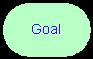
\includegraphics{media/imagenes/i_star/sintaxis/goal.jpg}
            \caption{Objetivo \gls{i*}}
            % \label{fig:my_label}
        \end{figure}

        \item Tareas: las tareas (\textit{Task}) son acciones que el usuario puede realizar para lograr su objetivo. Ejemplo: \guillemotleft Buscar pasajes de avión\guillemotright, \guillemotleft Comprar pasajes en la aerolínea\guillemotright.
        
        \begin{figure}[H]
            \centering
            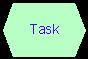
\includegraphics{media/imagenes/i_star/sintaxis/task.jpg}
            \caption{Tarea \gls{i*}}
            % \label{fig:my_label}
        \end{figure}
        \item Cualidades: o \textit{Qualities} son maneras o elementos de valor que se quiere preservar u obviar al completar un objetivo. Ejemplo: \guillemotleft Rápido\guillemotright, en esta serie de ejemplo la frase completa se entendería como \guillemotleft Tener los pasajes de avión comprados rápido\guillemotright o de manera \guillemotleft rápida\guillemotright.
                \begin{figure}[h]
            \centering
            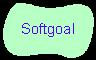
\includegraphics{media/imagenes/i_star/sintaxis/softgoal.jpg}
            \caption{Cualidad \gls{i*}, antes \textit{softgoal} en i* 1.0}
            % \label{fig:my_label}
        \end{figure}
        \item Recursos: Los recursos son elementos ligados a las tareas, como una \guillemotleft tarjeta de crédito\guillemotright en esa línea se podría \guillemotleft comprar los pases en la aerolínea con una tarjeta de crédito\guillemotright.
                \begin{figure}[h]
            \centering
            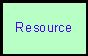
\includegraphics{media/imagenes/i_star/sintaxis/resource.jpg}
            \caption{Recurso \gls{i*}}
            % \label{fig:my_label}
        \end{figure}
        
        \item Actores: Los actores son elementos principales del diagrama, realiza acciones, dispone los recursos y tiene objetivos. Pueden ser de tres tipos: un tipo general cuando no se desea especificar, un agente que representa una instancia particular de un actor: como \guillemotleft Juan\guillemotright o el\guillemotleft Bot\guillemotright y un rol, que viene a ser una categoría o clase como \guillemotleft Estudiante\guillemotright.  Las \textit{boundaries} o límites relativos a un actor determinan que elementos le \guillemotleft pertenecen\guillemotright.
        
        \begin{figure}[h!]
            \centering
            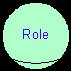
\includegraphics[scale=0.4]{media/imagenes/i_star/sintaxis/role.jpg}
            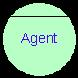
\includegraphics[scale=0.4]{media/imagenes/i_star/sintaxis/agent.jpg}
            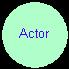
\includegraphics[scale=0.4]{media/imagenes/i_star/sintaxis/actor.jpg}
            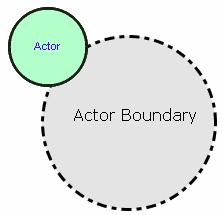
\includegraphics[scale=0.4]{media/imagenes/i_star/sintaxis/actorboundary.jpg}
            \caption{Actores \gls{i*}}
            % \label{fig:my_label}
        \end{figure}
        
        \item Enlaces: o \textit{Links} son lo que representa las relaciones entre los diferentes elementos del sistema, pueden representar dependencias, contribuciones, especificaciones o incluso notar una contribución. En el caso de este trabajo se usan principalmente 3 tipos de enlaces:
        \begin{itemize}

            \item Dependencias: Se indican con una letra D y expresan que el elemento a la izquierda de la dependencia, depende del elemento a la derecha, de manera un poco simplista.
            \begin{figure}[h!]
                \centering
                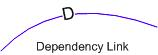
\includegraphics[scale=0.6]{media/imagenes/i_star/sintaxis/dependencylink.jpg}
                \caption{Dependencia \gls{i*}}
                % \label{fig:my_label}
            \end{figure}

            \item Contribuciones: Indican que cierto elemento contribuye a una Cualidad, puede ser de 4 formas, satisfaciendo completamente lo que se nota con \textit{make} sobre el enlace, Imposibilitando su realización lo que se denota con \textit{break}, o ayudando un poco o debilitando un poco lo que se denota con \textit{help} y \textit{hurt} respectivamente.
            \begin{figure}[h!]
                \centering
                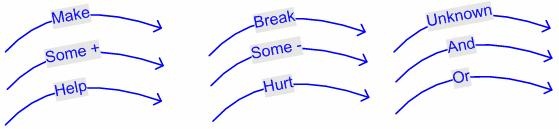
\includegraphics[scale=0.6]{media/imagenes/i_star/sintaxis/contribuitonlinks.jpg}
                \caption{Contribuciones \gls{i*}}
                % \label{fig:my_label}
            \end{figure}
            
            \item Refinamiento: Expresan que un objetivo o tarea tiene otros elementos que lo definen. Pueden ser O (\textit{OR}) o Y (\textit{AND}), lo que determinan es que para que el objetivo se satisfaga se debe satisfacer a su vez todos los elementos que lo refinan (\textit{AND}) o alguno de ellos (\textit{OR}).
            \begin{figure}[h!]
                \centering
                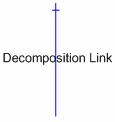
\includegraphics[scale=0.6]{media/imagenes/i_star/sintaxis/decomposition.jpg}
                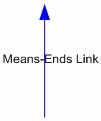
\includegraphics[scale=0.6]{media/imagenes/i_star/sintaxis/meansendslink.jpg}
                \caption{Refinamiento \gls{i*}}
                % \label{fig:my_label}
            \end{figure}
        \end{itemize}
    \end{itemize}
